\subsection{Simplified transformations}\label{sub:c3s1s2}
	\paragraph{}
	This subsection is concerned about discussing the simplifications that were added to the original transformations, that was explained in subsection \ref{sub:c3s1s1}. We will cover the following points in this subsection:
	\begin{itemize}
		\item The reason for doing such simplifications.
		\item What are the Simplifications.
		\item The resulted simplified transformations.
		\item Examples for the Output of the transformations, or let's name it Intermediate Output.
		\item Discussion on the Output of the prover.
	\end{itemize}

	\subsubsection{The Reason for doing the simplifications}
		\paragraph{}
		As mentioned before in subsection \ref{sub:c3s1s1}, the original transformations is generic for all sub-classes of \ac{fol}. So naturally it contains many steps that deals with proper function symbols. However, what concerns us in this project is only the \ac{epr} sub-class of problems. And by keeping in mind the definition of \ac{epr} as mentioned here in \ref{sub:c2s1s4}, and by knowing that there is no existence of proper function symbols, and that there won't be even after the skolemization step in any \ac{epr} problem, So implementing the original transformations, as they were, didn't seem logical as it won't be used in any of the problems, and it would take much more time to implement it practically. So those were the motives for having such simplifications.
	
	\subsubsection{What are the steps of the simplifications}
		\paragraph{}
		The simplifications made were very simple, and they were applied to all procedures of the original transformations. The steps of the simplifications are:
		
			\begin{enumerate}
				\item Every step that only deals with proper function symbols is removed since they are not existing in \ac{epr}. Ex.: some steps in \ac{crr} and \ac{rr} that loops on all the proper function symbols in the given problem.
				\item Any step or procedure that was introduced because of the existence of proper function symbols in problems were removed as well. Ex.: \ac{bs}, \ac{pf}, and \ac{bl}.
			\end{enumerate}
		
	\subsubsection{The resulted simplified transformations}
		\paragraph{}
		After applying the simplifications to the procedures of the transformations, the following steps were the only needed:
			
			\begin{itemize}
				\item Some steps in \ac{crr}.
				\item Some steps in \ac{rr}.
			\end{itemize}
		
		\paragraph{}
		For a chart representing the original \ac{crr} and what is removed from it, you can view figure ~\ref{fig:crr_b_and_a}, while figure ~\ref{fig:rr_b_and_a} is for \ac{rr}. And for a detailed explanation for the steps, you can check \cite{BMUG06}. 
		

			\begin{figure}[H]
				\centering
				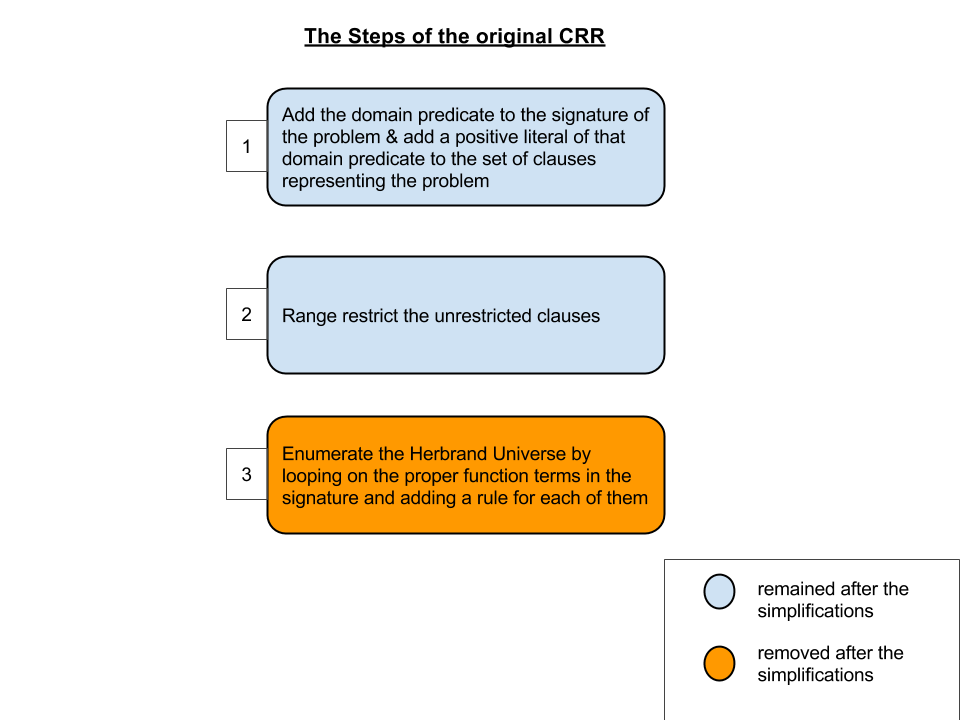
\includegraphics[scale=0.42]{pictures/crr_before_and_after.png}
				\caption{Original CRR with the kept and removed steps after the simplifications\label{fig:crr_b_and_a}}
			\end{figure}					  	

			\begin{figure}[H]
				\centering
				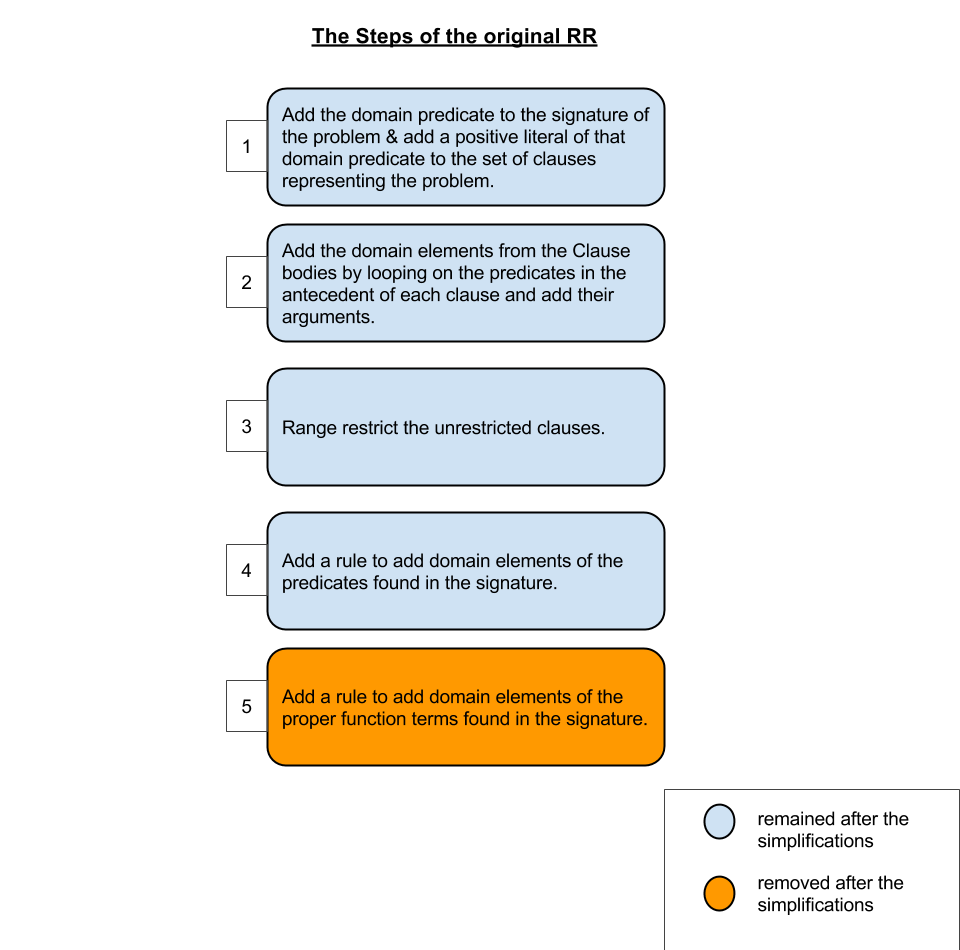
\includegraphics[scale=0.42]{pictures/rr_before_and_after.png}
				\caption{Original RR with the kept and removed steps after the simplifications\label{fig:rr_b_and_a}}
			\end{figure}
			

	\subsubsection{The Intermediate output}
		\paragraph{}
		Here we name the output of applying the simplified transformations on a set of (counter) satisfiable set of clauses an \textbf{Intermediate output}, since the Output should be the returned explicit (counter) model. So In this part we give an example for a problem, and then show what is the Intermediate output of that problem from \ac{crr}, and \ac{rr}. 		
		
		
		\paragraph{}
		It is notable to say that the following examples follow the TPTP CNF syntax. Moreover, the $\sim$ sign is used for negation, while the $\mid$ sign represents an or sign.
			
			\begin{minipage}{\textwidth}
			\begin{lstlisting}[caption=Satisfiable CNF problem Example,frame=single]
	cnf(agatha,axiom,(~lives(a))).
	cnf(butler,axiom,(dies(X)
			  |dies(Y)
			  |~lives(a)
			  |~lives(Y))).		
			\end{lstlisting}		
			
			\begin{lstlisting}[caption=CRR output Example,frame=single]
	cnf(i_0_1,axiom,(~lives(a))).
	cnf(i_0_2,axiom,(dies(X1)|dies(X2)
			  |~lives(a)|~lives(X2)
			  |~dom(X1))).
	cnf(i_0_3,plain,(dom(a))).
			\end{lstlisting}		

			\begin{lstlisting}[caption=RR output Example,frame=single]
	cnf(i_0_1,axiom,(~lives(a))).
	cnf(i_0_2,axiom,(dies(X1)|dies(X2)
			  |~lives(a)|~lives(X2)
			  |~dom(X1))).
	cnf(i_0_3,plain,(dom(a))).
	cnf(i_0_4,plain,(dom(a)|~lives(X1))).
	cnf(i_0_5,plain,(dom(a)|~lives(X2))).
	cnf(i_0_6,plain,(dom(X4)|~lives(X4))).
	cnf(i_0_7,plain,(dom(X5)|~dies(X5))).
			\end{lstlisting}		
			\end{minipage}
		

	\subsubsection{Discussion on the Output of the prover}
		\paragraph{}
		After applying the transformations on the clauses of a given problem, then this Intermediate output should be given as input to the normal proof procedure in E. And the final output for a (counter) satisfiable problem should be the saturated set, from which the explicit model should be extracted easily. However, this wasn't the case while running the problems, and the explicit model wasn't clear in the saturated set.
		
		\paragraph{}
		So a Model Construction Technique for resolution-based theorem provers was applied to the saturated set. And that Technique will be discussed in the following section \ref{sec:c3s2}.